% Template for ICIP-2010 paper; to be used with:
%          spconf.sty  - ICASSP/ICIP LaTeX style file, and
%          IEEEbib.bst - IEEE bibliography style file.
% --------------------------------------------------------------------------
\documentclass{article}
\usepackage{spconf,amsmath,graphicx}

% Example definitions.
% --------------------
\def\x{{\mathbf x}}
\def\L{{\cal L}}

% Title.
% ------
\title{LIGHTWEIGHT 3D MODELING OF URBAN BUILDINGS FROM RANGE DATA}
%
% Single address.
% ---------------
\name{Weihong Li, George Wolberg and Siavash Zokai}
\address{The City College of New York, Dept of Computer Science\\
	 138th Street at Convent Avenue, New York, NY, 10031 USA}
%
% For example:
% ------------
%\address{School\\
%	Department\\
%	Address}
%
% Two addresses (uncomment and modify for two-address case).
% ----------------------------------------------------------
%\twoauthors
%  {A. Author-one, B. Author-two\sthanks{Thanks to XYZ agency for funding.}}
%	{School A-B\\
%	Department A-B\\
%	Address A-B}
%  {C. Author-three, D. Author-four\sthanks{The fourth author performed the work
%	while at ...}}
%	{School C-D\\
%	Department C-D\\
%	Address C-D}
%

\newcommand{\Eq}[1] {Eq.~(\ref{eq:#1})}
\newcommand{\Fig}[1]{Fig.~\ref{fig:#1}}
\newcommand{\Sec}[1]{Sec.~\ref{sec:#1}}
\newcommand{\Eqs}   {Eqs.~}
\newcommand{\Figs}  {Figs.~}
\newcommand{\Tbl}[1]{Table~\ref{tbl:#1}}
\newcommand{\Etal}  {{\it et al.}}
\newcommand{\Figa}[1]{Fig.~\ref{fig:#1}(a)}
\newcommand{\Figb}[1]{Fig.~\ref{fig:#1}(b)}
\newcommand{\Figc}[1]{Fig.~\ref{fig:#1}(c)}
\newcommand{\Figd}[1]{Fig.~\ref{fig:#1}(d)}

\graphicspath{{figures/}}


\begin{document}
%\ninept
%
\maketitle
%
\begin{abstract}
Laser range scanners are widely used to acquire accurate scene measurements.
The massive point clouds they generate, however, present challenges to
efficient modeling and visualization.
We present an efficient modeling algorithm that exploits \emph{a priori}
knowledge that buildings can be modeled from cross-sectional contours
using extrusion and taper operations.
Inspired by this simple workflow, we identify key cross-sectional slices among
the point cloud.
Standard image processing algorithms are used to remove noise, fill holes,
and vectorize the projected points into planar contours.
Applying extrusion and taper operations to these contours
permits us to achieve dramatic geometry compression, making the resulting
models suitable for web-based applications such as Google Earth
or Microsoft Virtual Earth.
We present experimental results on the exterior and interior of urban building
datasets to validate the proposed algorithm.
\end{abstract}
%
\begin{keywords}
3D modeling, urban buildings, range data, point clouds, geometry compression
\end{keywords}
%
\section{INTRODUCTION}
\label{sec:intro}

Automatic 3D modeling of urban buildings is an area of active research
with increasing attention drawn from the computer graphics and
computer vision communities.
Current state-of-the-art algorithms for 3D modeling of urban buildings are
computationally expensive and suffer under the weight of large-scale datasets.
Despite a recent thrust of activity in 3D modeling and visualization of
urban buildings for web-based applications such as Google Earth and Microsoft
Virtual Earth, much 3D modeling continues to be manually generated.
This paper seeks to introduce an automatic and efficient algorithm for
generating lightweight 3D models of urban buildings directly from point clouds.

In an attempt to steer clear of tedious and expensive hand-made models,
procedural modeling of buildings in \cite{PMB_MWH,PMB_WWS} has been proposed.
By using an effective description language, buildings and streets of a virtual
city can be generated automatically.
However, since the parameters used to generate the buildings are randomly
generated, the city generated with these buildings and streets is a virtual one.
This approach is not useful for attempting to model an {\it existing} building.

We propose an efficient way to reconstruct 3D models from range data by
partitioning the data into thin cross-sectional slabs of volume.
An overview of our approach, depicted in \Fig{ov}, begins with the
acquisition of a dense 3D point cloud $C$ of a building.
$C$ is then partitioned into a nonoverlapping set of volumetric slabs.
Each slab $S$ is associated with one projection plane $P$,
sitting at the base of $S$.
The purpose of partitioning $C$ is to establish a set of cross-sections,
or contour slices.
By examining the changes among these slices, we can identify the prominent
slices, or {\it keyslices}, as well as the necessary extrusion and
taper operations that must apply to them to generate the model.
By casting this 3D modeling task into a series of 2D operations, we
reduce the dimension of the problem to achieve a significant savings in
computational complexity.

\begin{figure*}[htbp]
\begin{center}
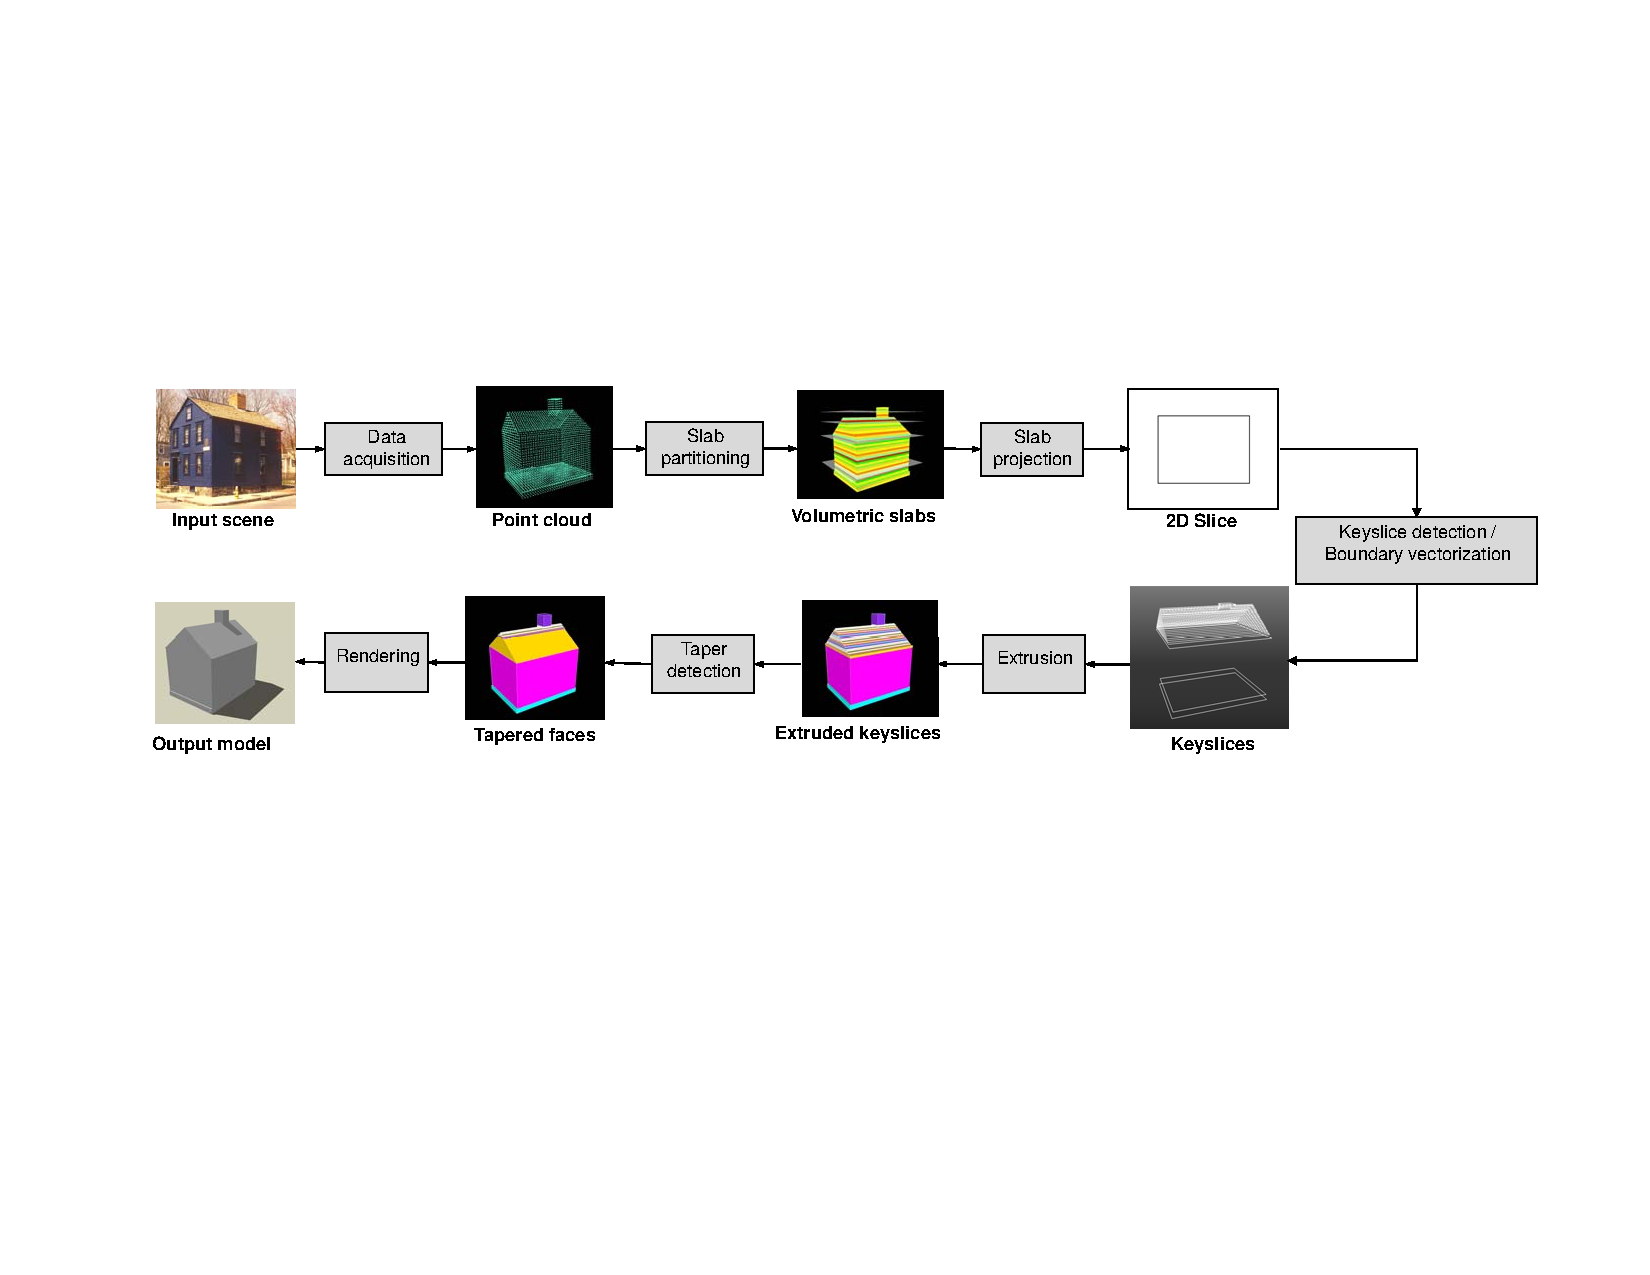
\includegraphics[width=7in]{overview.pdf}
\end{center}
\caption{Overview of the proposed approach.}
\label{fig:ov}
\end{figure*}

\section{PREPROCESSING THE RANGE DATA}
\label{sec:prepdata}

The input to our system is range data assembled as a 3D point cloud.
Our data is obtained from a Leica Cyrax 2500 laser range scanner \cite{RDP_LRS},
which works by sweeping an eye-safe laser beam across the scene to collect
up to one million 3D depth points per frame.
All scene points that lie within 100 meters can be acquired with an accuracy
of 5mm in depth.
The basic algorithm that we use for registering the voluminous 3D data
acquired from multiple scans of buildings has been introduced in
\cite{RDP_LS}.
That same algorithm is also responsible for extracting the major axes
of the building in order to align it to the axes of the world coordinate
system.
This is necessary to properly infer the keyslices.

We consider the point cloud data as a large array of 3D points to be
sliced into horizontal volumetric slabs.
All 3D points within each slab are projected onto a horizontal projection
plane, or slice, at the base of the slab.
The 3D points in each slab are projected onto a projection plane to
form cross-sectional contour slices.
\Fig{slicing} depicts four such slices.
The height of each slab is $\boldsymbol{\delta}$.
If $\boldsymbol{\delta}$ is held constant, each slice is generated from
equi-spaced slab intervals.
If $\boldsymbol{\delta}$ is allowed to vary, then we may
choose to allow for large values in parts of the structure that are similar,
and low values in regions that contain finer detail.
To avoid working on 3D data directly, a relatively small constant value
for $\boldsymbol{\delta}$ is chosen to generate 2D cross-sectional image slices.

\begin{figure} [htbp]
\begin{center}
\begin{tabular}{cc}
\fbox{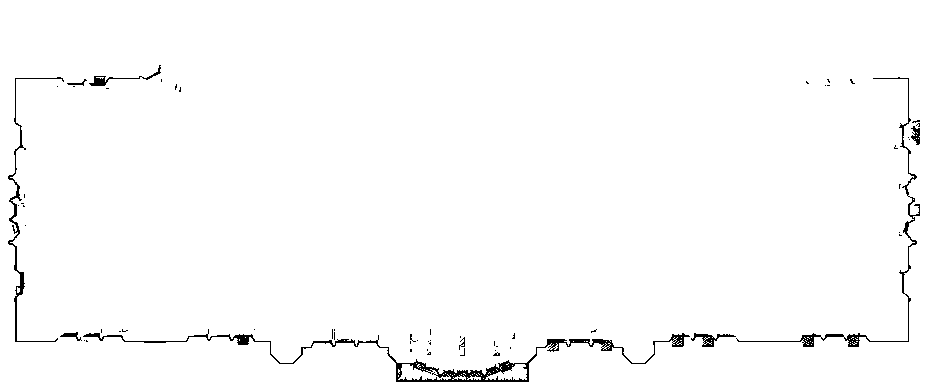
\includegraphics[width=0.2\textwidth]{image_slice_0190.png}} &
\fbox{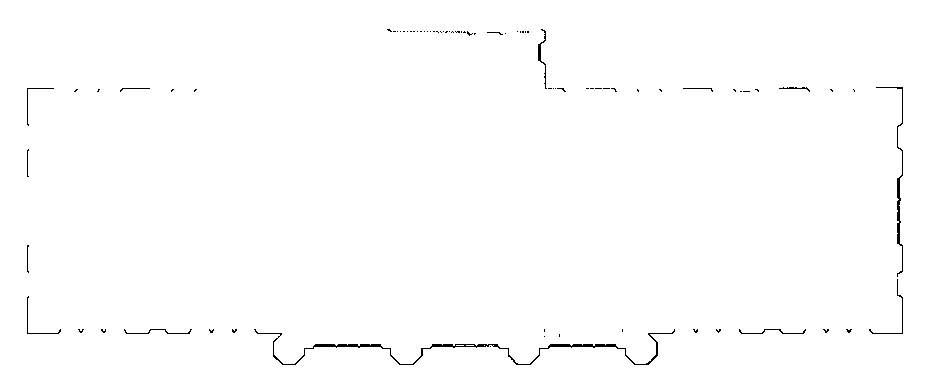
\includegraphics[width=0.2\textwidth]{image_slice_0600.png}} \\
(a) & (b) \\
\fbox{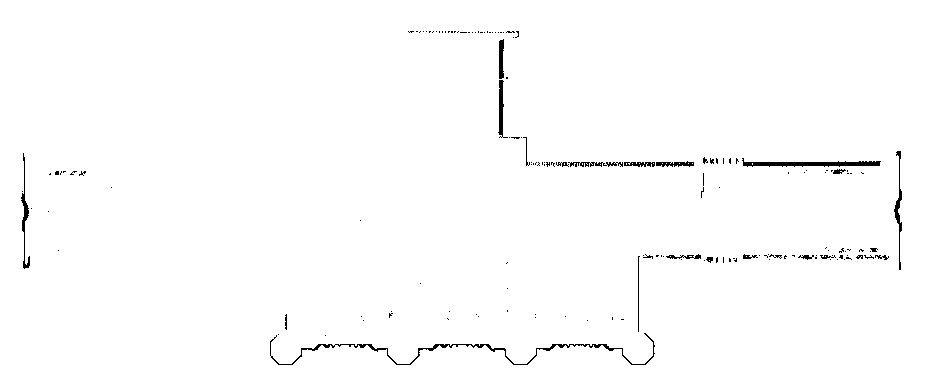
\includegraphics[width=0.2\textwidth]{image_slice_0714.png}} &
\fbox{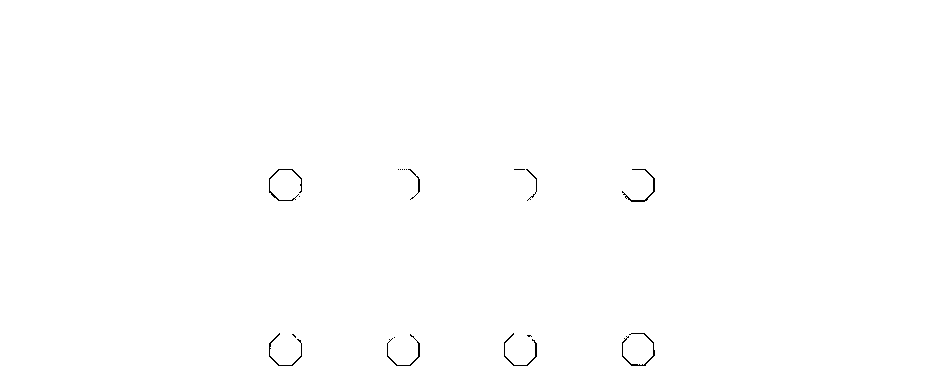
\includegraphics[width=0.2\textwidth]{image_slice_0951.png}} \\
(c) & (d)
\end{tabular}
\end{center}
\caption{The set of slices corresponding to the four projection planes of
different heights.}
\label{fig:slicing}
\end{figure}

Without loss of generality, the $y-$axis is used to represent the bottom-up
vertical direction.
Over each slab in height range $[H_{lo}, H_{hi})$,
we project the 3D data $\boldsymbol{P}(x,y,z)$, for $H_{lo} \leq y < H_{hi}$,
onto a 2D image slice.
The projection is normalized in the range $[0,W]$, where $W$ is the image width:
\begin{equation}
[\,x^{2D},\; y^{2D}\,]^T = \omega\cdot[\,x^{3D}_i - X_{MIN},\; z^{3D}_i - Z_{MIN}\,]^T
\label{eq:image_slicing}
\end{equation}
Note that $\omega = W/(X_{MAX} - X_{MIN})$, and that
the [$X_{MIN}$, $X_{MAX}$] and [$Z_{MIN}$, $Z_{MAX}$] pairs define the
3D bounding box, which can be obtained through user input and can be used
to clip away noise data.
\Fig{slicing}(a)-(d) show some examples of the 2D slices, where noise
and incomplete data are observed.

The slices we extract above often have holes (i.e., missing data) due to
occlusion or other visibility issues.
Fortunately, most urban buildings have symmetry that we can exploit to
fill these holes.
Symmetry computation on 3D data \cite{Sym_PSGRF,Sym_ZPA} is expensive,
so we conduct this computation on the 2D image slices.
Since the 3D data has been already rectified \cite{RDP_LSYGS} and projected onto 2D slices, 
hence only 2D translation
is needed to be considered for symmetry computation.
Let $P(x,y)$ be a point on the original image $I$ and $P'(x',y')$ be the reflected
point of $P$ with respect to a symmetry line $L$.
The symmetry computation equation for $L$ is as follows:
\begin{equation}
L = \underset{x,y}{\operatorname{arg\,min}}\sum{d_{x,y}(P', I)}
\end{equation}
where the $d_{x,y}(P',I)$ is the distance between the self-reflected point
$P'$ and its nearest data point in image $I$.
The reflected point $P'$ of the original point $P$ is computed with
respect to a line along either the $x-$ or $y-$ axis.
Therefore, the symmetry line $L$ is obtained as the line with minimum
summation error over the reflected data points.

%%%%%%%%%%%%%%%%%%%%%%%%%%%%%%%%
%%%%%%   3D Reconstruction  %%%%
%%%%%%%%%%%%%%%%%%%%%%%%%%%%%%%%
\section{LIGHTWEIGHT 3D RECONSTRUCTION}
\label{sec:reconst}

Our 3D modeling algorithm is based on \emph{a priori} knowledge that
urban buildings can be created through a series of extrusion and taper
operations on the salient cross-sections contained in the keyslices.
The key step for successful modeling is identifying these salient cross
sections upon which the extrusion and taper operations will apply.

\subsection{Keyslice Detection}
\label{ssec:ksd}
The 2D image slices of an extruded region are similar to each other.
Thus, to detect the keyslices that delimit extruded regions, one only needs
to compute the similarity between adjacent slices based on an
objective distance function.
Let $P_r(x_r, y_r)$ be a data point in a reference image and
let $P_i(x_i, y_i)$ be a data point in a new observed image $I$.
We defined the following objective distance of image $I$ to reference image $I_r$
for the similarity measure:

\begin{equation}
d_H(I, I_r) = \sum_{i=0}^Nd_{min}(P_i, I_r)
\label{eq:hd}
\end{equation}

where $d_{min}(P_i, I_r)$ is the minimum distance from data point $P_i$
in image $I$ to the reference image $I_r$.
This distance function is similar to Hausdorff distance.
To compute the keyslices, a threshold $\tau_{d}$ is used for the
distance function $d_{HD}$.
If $d_{HD} < \tau_{d}$, the two images $I$ and $I_r$ are considered
similar to each other.
Otherwise, a keyslice image is found and $I_r$ is updated with $I$,
the new keyslice image.

The accuracy of the keyslices detected by using this distance function
is closely tied to threshold $\tau_d$.
Small $\tau_d$ leads to more accurate models but requires more time and
space to compute and store the result.
Large $\tau_d$ tends to be time and space efficiency but 
ends up with coarse models which might potentially
miss some salient structures or features.
By default, we set $\tau_d$ to be 4 (pixels), which shows good balance
between accuracy and computational efficiency for our experiments. 

\subsection{Boundary Vectorization}
\label{ssec:BPA}

After the keyslices are detected, $N_K$ keyslices will be identified
from a total of $N_A$ image slices.
To generate the 3D model, these keyslice images need to be vectorized to
represent the contours of the building facade.
We adapted the ball-pivoting algorithm (BPA)
\cite{BPA_BMRS} from its original use on 3D point cloud data to use on
2D keyslice images where it produces vectorized boundaries.
The key parameter for the BPA algorithm to work successfully is to
find the right size of the ball for pivoting.
We propose a coarse-to-fine adaptive BPA algorithm, described below,
to solve this problem.

\begin{figure}[hbtp]
\centering
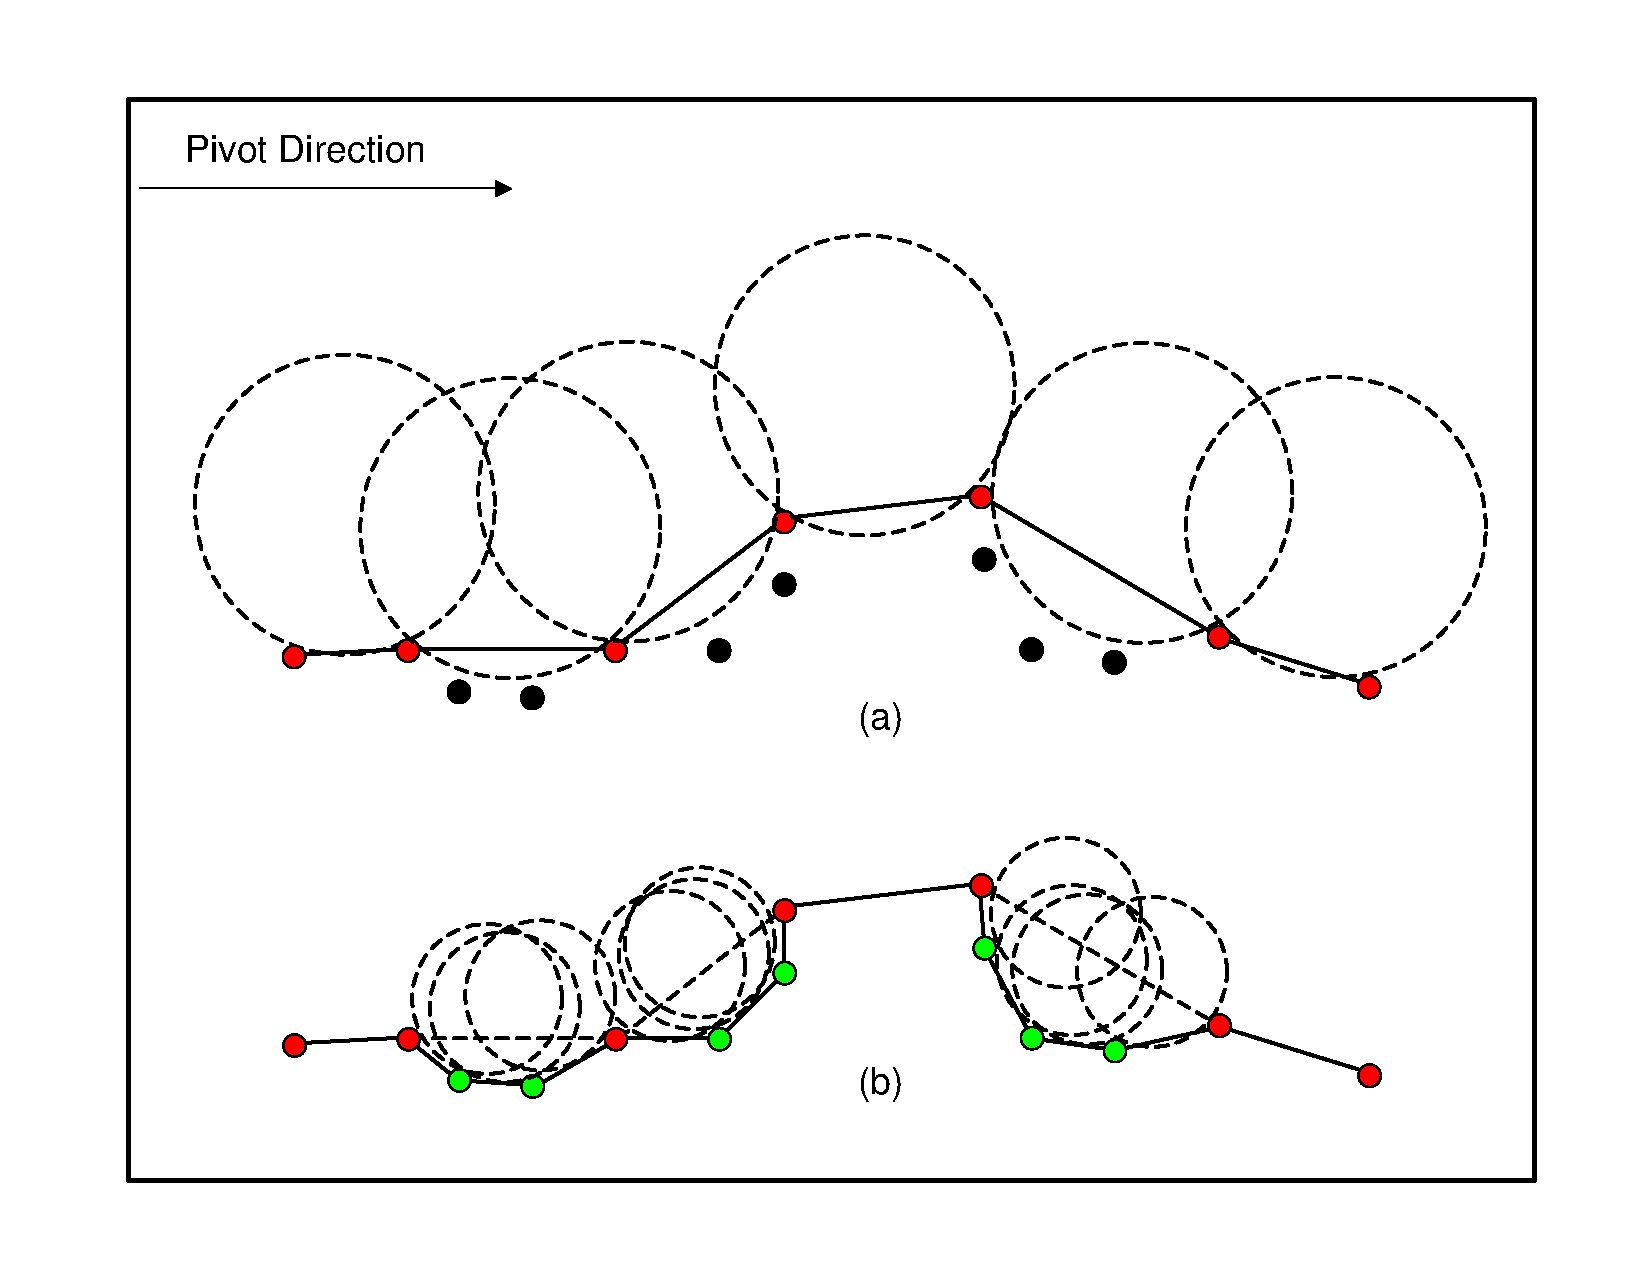
\includegraphics[width=0.25\textwidth]{figures/BPA.pdf}
\caption{Adaptive ball pivoting algorithm:
(a) Initial pivoting with circle of radius 2$r$;
(b) Refinement with circle of radius $r$.}
\label{fig:BPA}
\end{figure}

Due to the gap between data points, a relatively large radius $r$ is chosen
as a coarse step to ensure that the ball will travel across all boundary
data before turning back or reaching any existing boundary points.
\Figa{BPA} shows an initial ball-pivoting process on 2D data points.
The output of the initial BPA $\boldsymbol{\Phi}$ contains an ordered list of the boundary data
points $\boldsymbol{P}$ and their corresponding directions $\overrightarrow{\boldsymbol{R}}$ in which
the circle $C$ starts pivoting.
The iterative BPA refinement process applies a smaller radius, e.g., $r' = r/2$,
to $\boldsymbol{\Phi}$ to get more accurate results, as shown in \Figb{BPA}.
The length of each line segment formed by adjacent points is checked,
$\ell = \overline{P_0P_1}$, in $\boldsymbol{\Phi}$.
If this line is long enough, the BPA is applied between the two adjacent points.
When the ball reaches the second point, a new list of ordered boundary points,
$\boldsymbol{\Phi'}$, is inserted into $\boldsymbol{\Phi}$ between $P_0$ and
$P_1$.
This process continues until it finishes checking every adjacent point in $\boldsymbol{\Phi}$.
The refinement stops when $r'$ falls below threshold $\tau_r$.
 
\subsection{Tapered Structure Detection}
\label{sec:tsd}

After the keyslices are detected and vectorized, the contours of
$N_K = \{I_{i}, i = 0, ..., K \}$ keyslices are used to represent
the building based on the extrusion operation.
That is, the space between each pair of keyslices, say $I_{i}$ and $I_{j}$,
can be interpolated by the lower keyslice, e.g., $I_{i}$ in this case.
This is valid due to the similarity between the intermediate slices
and the keyslice $I_{i}$.

\begin{figure}[htbp]
\begin{center}
\begin{tabular}{cc}
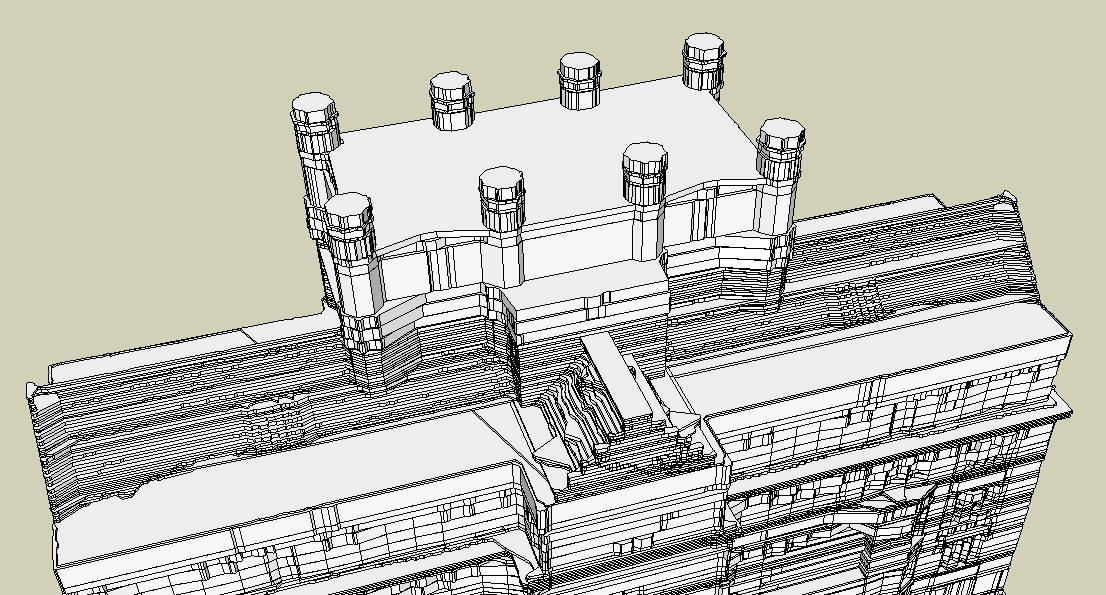
\includegraphics[width=0.2\textwidth]{extrude_1.png} &
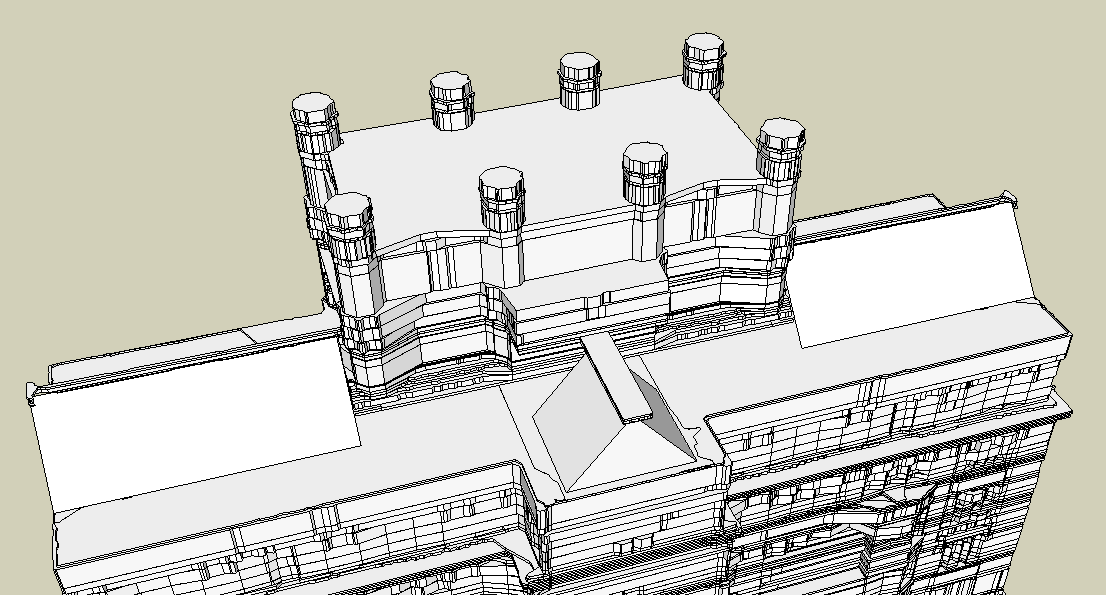
\includegraphics[width=0.2\textwidth]{extrude_2.png} \\
(a) & (b)
\end{tabular}
\end{center}
\caption{The top view of the 3D building shown (a) without tapered structures
and (b) with tapered structures.}
\label{fig:DXF_top}
\end{figure}

In addition to the extrusion operation, we can further improve the model
and reduce the model size by the observation that some of keyslice images
belong to the same tapered structure, as demonstrated in \Fig{DXF_top}.
\Figa{DXF_top} shows the roof structure
of the reconstructed model based on a keyslice image extrusion operation with
almost half of the keyslice images dedicated to the structure.
After inferring the tapered structure, \Figb{DXF_top} shows the improvement
of the modeling, which is smoother than the previous model.
In addition, the keyslices needed to represent the building, and its
associated storage, are reduced almost in half.

The difficulty in inferring tapered structures lies on the 
mixed layout of tapered and extruded structures, as depicted in \Figa{DXF_top}.
Our solution is based on the divide-and-conquer strategy:
the whole structure $\boldsymbol{U}$ is segmented into independent
sub-structure units, $U_0, U_1, \ldots, U_N$.
Any sub-structure unit $U_i$ is constrained to contain a unique structure,
i.e., either a tapered or an extruded one.
Once each unit $U_i$ is inferred, the whole structure can be modeled by a
union operation of these sub-structures, i.e.,
$\boldsymbol{U} = \bigcup{U_i\{ i = 1,\ldots,N\}}$.



%%%%%%%%%%%%%%%%%%%%%%%%%%%%%%%%
%%%%%%   Experimental Results%%%
%%%%%%%%%%%%%%%%%%%%%%%%%%%%%%%%
\section{EXPERIMENTAL RESULTS}
\label{sec:IR_OUT}

\begin{figure}[htbp]
\begin{center}
\begin{tabular}{cc}
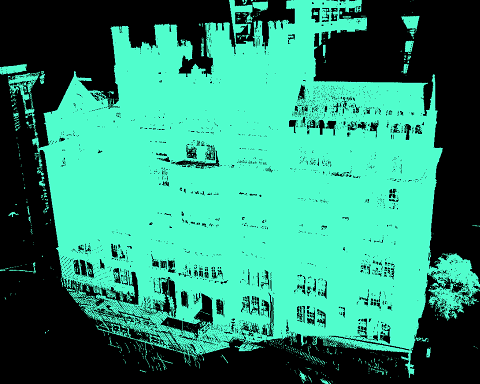
\includegraphics[width=0.22\textwidth]{point_cloud.png} &
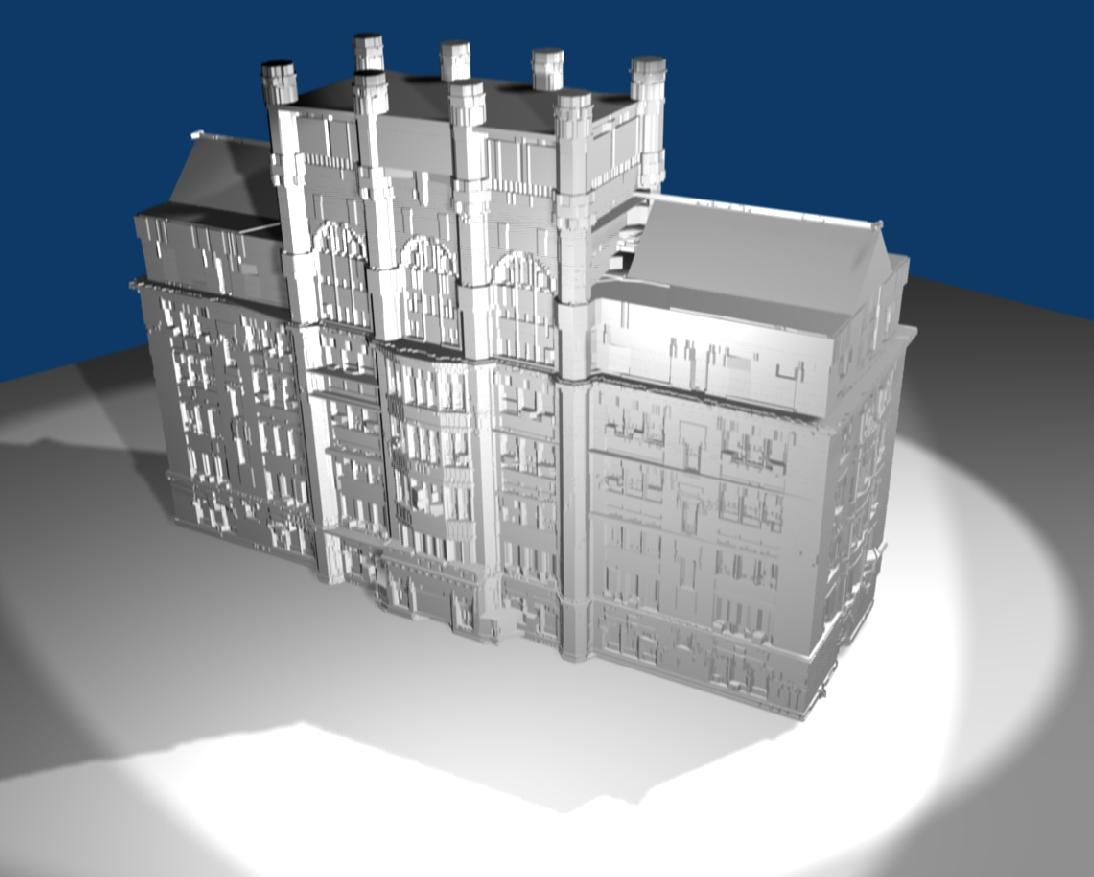
\includegraphics[width=0.22\textwidth]{HunterShaded.jpg} \\
(a) & (b) \\
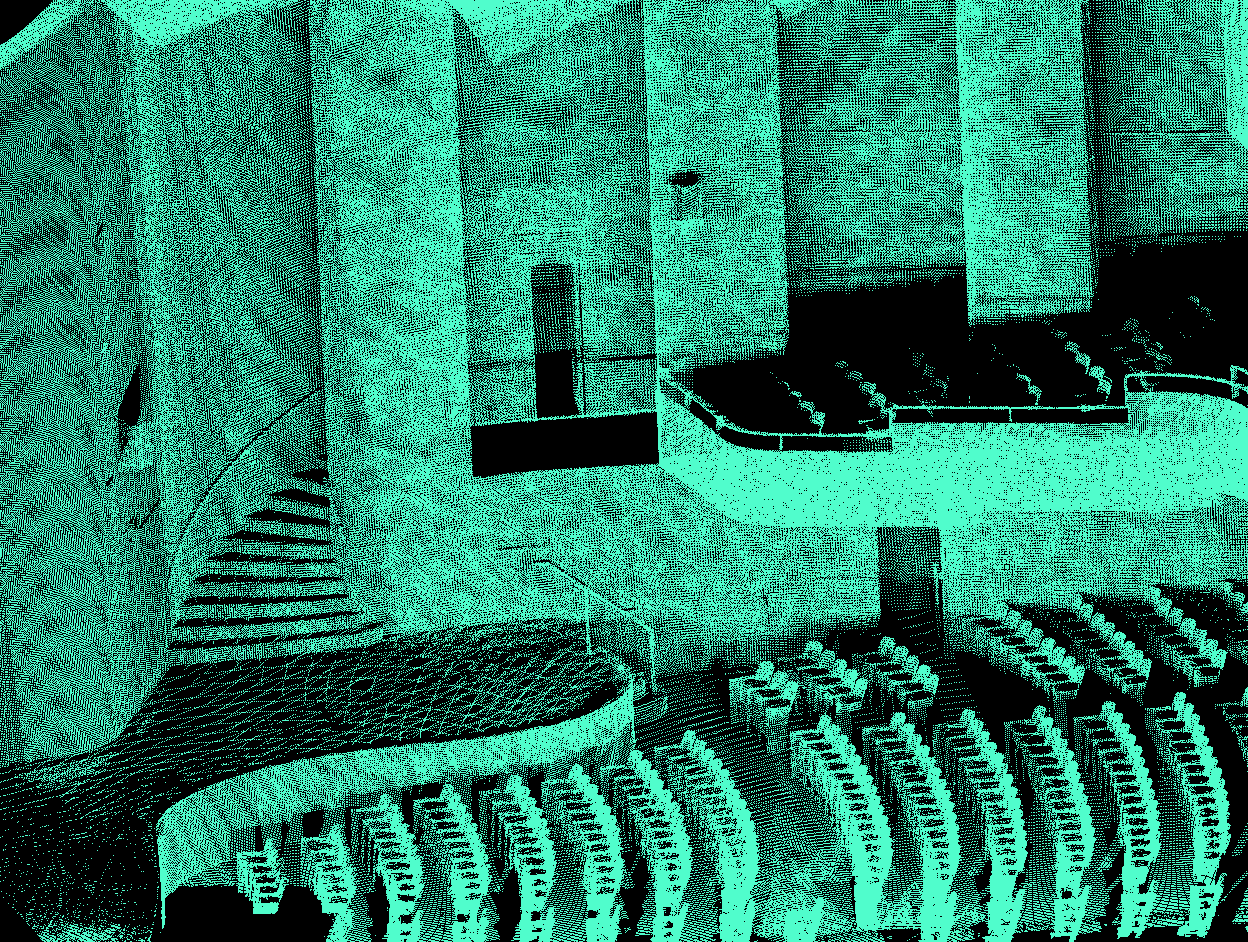
\includegraphics[width=0.22\textwidth]{range_crop.png} &
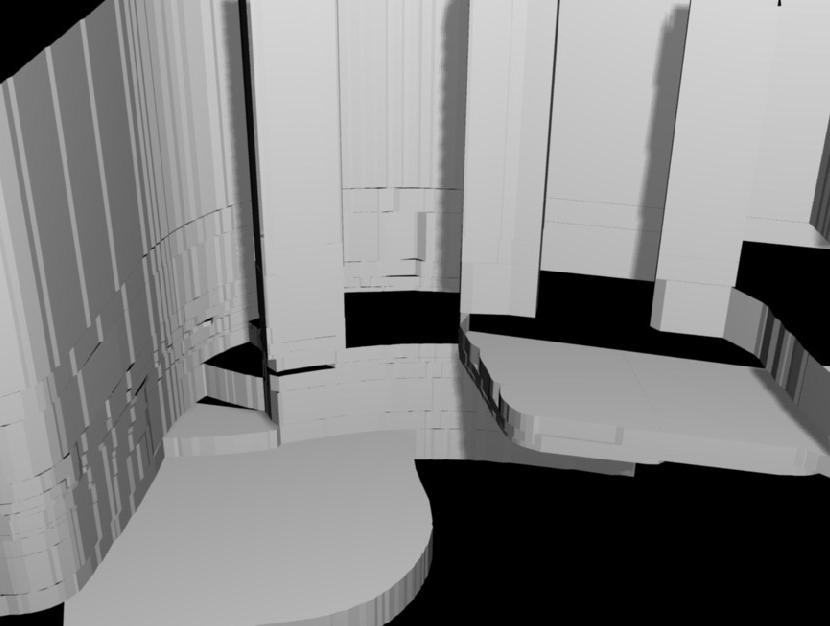
\includegraphics[width=0.22\textwidth]{HunterTheatreShaded.jpg} \\
(c) & (d)
\end{tabular}
\end{center}
\caption{The model of scans. (a) Point cloud data and the
(b) reconstructed lightweight 3D model for an exterior scan.
(c) Point cloud data and the
(d) reconstructed lightweight 3D model for an interior scan.}
\label{fig:IN}
\end{figure}

After obtaining the extrusion and tapered structures, 
We can easily transform these in 2D image system back to the 3D to generate final models.
\Figb{IN} shows an exterior 3D model generated by the above
transformation after rendering.
The snapshot of an interior scan of a theater is shown in \Figc{IN}
and its reconstructed 3D model is shown in \Figd{IN}.
This model is primarily reconstructed using the extrusion unit
upon the main structures of the interior.
The chairs and some other fine details were manually culled.

\Tbl{em} lists the relationship among the $\tau_d$, errors,
number of faces, and model size for the input data in \Figa{IN}.
The units for $\tau_d$ and error is in pixels and millimeters, respectively.
The size of the original point cloud for the 3D building is more than 700 MB.
From the table, one can see that even for the most accurate model, the size
is dramatically reduced compared with the original 3D point cloud data.
This is a desirable property for web-based applications.
The low resolution ($\tau_d = 64$) and high resolution ($\tau_d = 4$) models
were generated in 10 and 40 minutes, respectively,
on a laptop PC running an Intel Core 2 T7200 CPU at 2.0 GHz with 2.0 GB RAM.

\setlength{\tabcolsep}{4pt}
\begin{table}[hbtp]
\begin{center}
\begin{tabular}[t]{||c||c|c|c||}
\hline
$\tau_{d} $(pixel) & Error (mm)& \# of faces & Size (KB) \\ \hline \hline
64 & 0.658 & 1471  & 15  \\ \hline
32 & 0.294 & 3284  & 32  \\ \hline
16 & 0.141 & 8574  & 86  \\ \hline
8  & 0.131 & 13955 & 137 \\ \hline
4  & 0.094 & 27214 & 261 \\ \hline
2  & 0.088 & 31331 & 335 \\ \hline
1  & 0.083 & 32187 & 337 \\ \hline
\end{tabular}
\end{center}
\caption{Error measurements for reconstruction of \Figa{IN} using
the BPA radius threshold $\tau_r = 4$.}
\label{tbl:em}
\end{table}
\setlength{\tabcolsep}{1.4pt}

%%%%%%%%%%%%%%%%%%%%%%%%%%%%%%%%
%%%%%%   Conclusion and Future Work%%%
%%%%%%%%%%%%%%%%%%%%%%%%%%%%%%%%
\section{Conclusion}

This paper has presented an efficient algorithm for lightweight 3D modeling
of urban buildings from range data.
Our work is based on the observation that buildings can be viewed as the
combination of two basic components: extrusion and tapering.
The range data is partitioned into volumetric slabs whose 3D points are
projected onto a series of uniform cross-sectional planes.
Experimental results on both exterior and interior urban building datasets
have been presented to validate the proposed approach.

There are some limitations for the proposed approach. 
Although the reconstructed model is good enough for web-based applications,
the accuracy would reach a bottleneck when the threshold $\tau_d$ and $\tau_r$ decreased to
certain small value. On the other hand, this approach is sensitive on 
the result of the registration and rectification of the laser scans. 
In other words, the inaccuracy of the major axes computation would impose problems for
the 3D slabs projection and the following model reconstruction algorithms.

%\section{ILLUSTRATIONS, GRAPHS, AND PHOTOGRAPHS}
%\label{sec:illust}
%
%Illustrations must appear within the designated margins.  They may span the two
%columns.  If possible, position illustrations at the top of columns, rather
%than in the middle or at the bottom.  Caption and number every illustration.
%All halftone illustrations must be clear black and white prints.  Colors may be
%used, but they should be selected so as to be readable when printed on a
%black-only printer.
%
%Since there are many ways, often incompatible, of including images (e.g., with
%experimental results) in a LaTeX document, below is an example of how to do
%this \cite{Lamp86}.
%
%% Below is an example of how to insert images. Delete the ``\vspace'' line,
%% uncomment the preceding line ``\centerline...'' and replace ``imageX.ps''
%% with a suitable PostScript file name.
%% -------------------------------------------------------------------------
%\begin{figure}[htb]
%
%\begin{minipage}[b]{1.0\linewidth}
%  \centering
%  \centerline{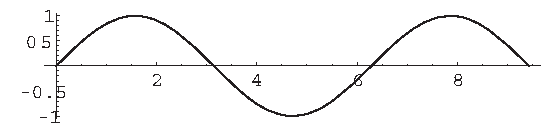
\includegraphics[width=8.5cm]{image1}}
%%  \vspace{2.0cm}
%  \centerline{(a) Result 1}\medskip
%\end{minipage}
%%
%\begin{minipage}[b]{.48\linewidth}
%  \centering
%  \centerline{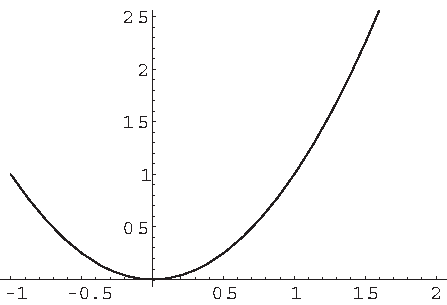
\includegraphics[width=4.0cm]{image3}}
%%  \vspace{1.5cm}
%  \centerline{(b) Results 3}\medskip
%\end{minipage}
%\hfill
%\begin{minipage}[b]{0.48\linewidth}
%  \centering
%  \centerline{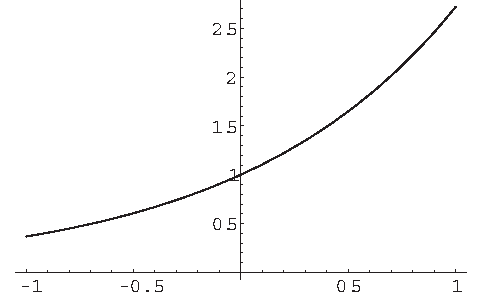
\includegraphics[width=4.0cm]{image4}}
%%  \vspace{1.5cm}
%  \centerline{(c) Result 4}\medskip
%\end{minipage}
%%
%\caption{Example of placing a figure with experimental results.}
%\label{fig:res}
%%
%\end{figure}
%
%
%% To start a new column (but not a new page) and help balance the last-page
%% column length use \vfill\pagebreak.
%% -------------------------------------------------------------------------
%\vfill
%\pagebreak
%
%
%\section{FOOTNOTES}
%\label{sec:foot}
%
%Use footnotes sparingly (or not at all!) and place them at the bottom of the
%column on the page on which they are referenced. Use Times 9-point type,
%single-spaced. To help your readers, avoid using footnotes altogether and
%include necessary peripheral observations in the text (within parentheses, if
%you prefer, as in this sentence).
%
%
%\section{COPYRIGHT FORMS}
%\label{sec:copyright}
%
%You must include your fully completed, signed IEEE copyright release form when
%you submit your paper. We {\bf must} have this form before your paper can be
%published in the proceedings.
%
%\section{REFERENCES}
%\label{sec:ref}
%
%List and number all bibliographical references at the end of the paper.  The references can be numbered in alphabetic order or in order of appearance in the document.  When referring to them in the text, type the corresponding reference number in square brackets as shown at the end of this sentence \cite{C2}.
%
%% References should be produced using the bibtex program from suitable
%% BiBTeX files (here: strings, refs, manuals). The IEEEbib.bst bibliography
%% style file from IEEE produces unsorted bibliography list.
%% -------------------------------------------------------------------------
\bibliographystyle{IEEEbib}
\bibliography{icip}

\end{document}
